\documentclass[svgnames]{beamer}


\mode<presentation>
{
  \usetheme[titleformat=smallcaps,numbering=fraction,progressbar=frametitle]{metropolis}
  \usecolortheme[light,accent=orange]{solarized}
  %\usecolortheme[named=Goldenrod]{structure}
  % or ...

  \setbeamercovered{transparent}
  % or whatever (possibly just delete it)
}


% \usepackage{mathtext}
\usepackage[utf8]{inputenc}
\usepackage[english,russian]{babel}
\usepackage{cmap}
\usepackage{amsmath}
\hypersetup{unicode=true}
\graphicspath{{images/}{slides/images}}


\title[QTA 06] % (optional, use only with long paper }
{Проклятие размерности. Регуляризация}

\subtitle
{Квантитативный анализ текста} % (optional)

\author%[Author, Another] % (optional, use only with lots of authors)
{Кирилл Александрович Маслинский}
% - Use the \inst{?} command only if the authors have different
%   affiliation.

\institute%[Universities of Somewhere and Elsewhere] % (optional, but mostly needed)
{НИУ ВШЭ Санкт-Петербург}
% - Use the \inst command only if there are several affiliations.
% - Keep it simple, no one is interested in your street address.

\date%[Short Occasion] % (optional)
{04.04.2022 / 06}

\subject{natural language processing, text mining}
% This is only inserted into the PDF information catalog. Can be left
% out. 



% If you have a file called "university-logo-filename.xxx", where xxx
% is a graphic format that can be processed by latex or pdflatex,
% resp., then you can add a logo as follows:

% \pgfdeclareimage[height=0.5cm]{university-logo}{university-logo-filename}
% \logo{\pgfuseimage{university-logo}}

% Delete this, if you do not want the table of contents to pop up at
% the beginning of each subsection:

\newcommand{\plate}[1]{\begingroup\setbeamercolor{background canvas}{bg=Beige}
  % \begin{frame}<beamer>{Outline}
  %   \tableofcontents[sectionstyle=show/hide,subsectionstyle=show/shaded/hide]
  % \end{frame}
  \begin{frame}[plain]
  \vfill
  \centering
  \begin{beamercolorbox}[sep=8pt,center,shadow=true,rounded=true]{title}
    \usebeamerfont{title}#1\par%
  \end{beamercolorbox}
  \vfill
  \end{frame}
  \endgroup
}

% \AtBeginSection[]
% {
%   \begin{frame}<beamer>[plain]{План}
%     \tableofcontents[sectionstyle=shaded,subsectionstyle=hide]
%   \end{frame}
% }

% \AtBeginSubsection[]
% {
%   \begin{frame}<beamer>[plain]{План}
%     \tableofcontents[sectionstyle=shaded,subsectionstyle=show]
%   \end{frame}
% }

\newcommand{\tb}[1]{\colorbox{yellow}{#1}\space}
\newcommand{\Sp}[1]{\colorbox{green}{#1}\space}
\newcommand{\Sn}[1]{\colorbox{red}{#1}\space}


\begin{document}

\begin{frame}
  \titlepage
\end{frame}

\section{Проклятие размерности}

\begin{frame}[fragile]
  \frametitle{Sparse data problem}
\begin{verbatim}
    Terms
Docs выгребать выгребной выгружать выгрузка выгрызать
   1         0         0         0        0         0
   2         0         0         0        0         0
   3         0         0         0        0         0
   4         0         0         0        0         0
   5         0         0         0        0         0
\end{verbatim}
\end{frame}

\begin{frame}[fragile]
  \frametitle{Проклятие размерности}
  \framesubtitle{Curse of dimensionality}
\begin{verbatim}
A document-term matrix (1530 documents, 13322 terms)

Non-/sparse entries: 68859/20313801
Sparsity           : 100%
Maximal term length: 66 
Weighting          : term frequency (tf)
\end{verbatim}
\end{frame}

\begin{frame}
  \frametitle{Hughes phenomenon}
  \centering
  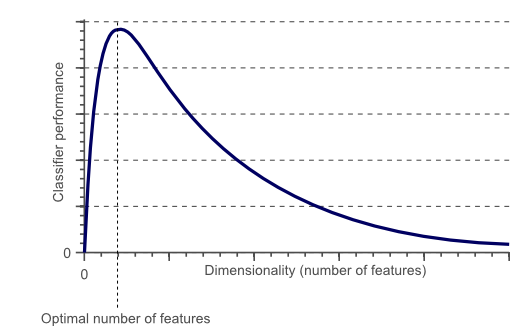
\includegraphics[width=.9\textwidth]{dimensionality_vs_performance}
\end{frame}

\begin{frame}
  \frametitle{Проклятие размерности на кошках}
  \centering
  \includegraphics<1>[width=.6\textwidth]{1Dproblem}
  \includegraphics<2>[width=.6\textwidth]{2Dproblem}
  \includegraphics<3>[width=.6\textwidth]{3Dproblem}
  \includegraphics<4>[width=.6\textwidth]{3Dproblem_separated}
\end{frame}

\begin{frame}
  \frametitle{Переобучение}
  \centering
  \includegraphics<1>[width=.6\textwidth]{overfitting}  
  \includegraphics<2>[width=.6\textwidth]{no_overfitting}  
\end{frame}


\section{Снижение размерности: простые способы}

\begin{frame}
  \frametitle{Снижение размерности}
  \begin{itemize}
  \item Матрица терминов-документов очень большая и редкая
  \item Близкие по смыслу слова не обязательно встречаются в одних и
    тех же документах:
    \begin{itemize}
    \item синонимия
    \item полисемия
    \item шум
    \end{itemize}
    \pause
  \item Нужно сократить размерность матрицы (сделать меньше столбцов).
  \end{itemize}
\end{frame}

\begin{frame}
  \frametitle{Стоп-слова}
Простейший способ уменьшить число столбцов — просто \alert{удалить
  лишние слова}:

  \begin{itemize}
  \item Статический список:

без
более
бы
был
была
были
было
быть
в
вам
вас
весь
во
вот
все
всего
всех
вы
где
да
даже
для ...

  \item Динамический список:

    \begin{itemize}
    \item Слишком частотные (N самых частотных)
    \item Слишком редкие (порог: не менее чем в F документов)
    \item Слишком короткие (меньше M букв)
    \end{itemize}
  \end{itemize}
\end{frame}

\section{Алгоритм классификации: Логистическая регрессия}

\begin{frame}
  \frametitle{Простая линейная регрессия}
  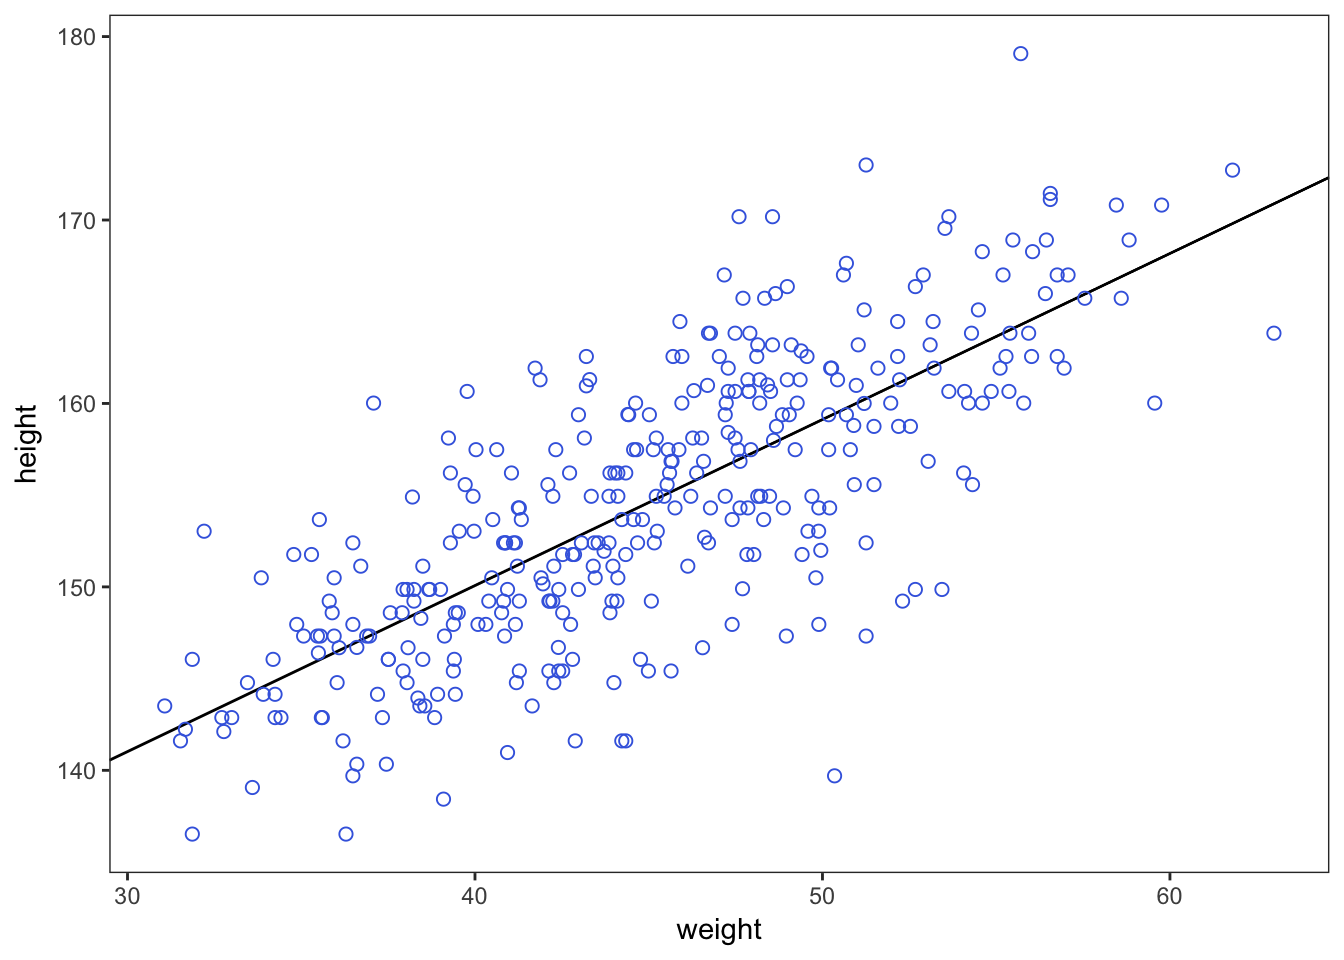
\includegraphics[width=\textwidth]{lin-regression}
\end{frame}

\begin{frame}
  \frametitle{Линейная регрессия: генеративная формулировка}
  \begin{columns}
    \column{.5\textwidth}
    \begin{equation}
      \begin{split}
        \label{eq:1}
        H_i \sim \mathcal{N}(\mu_i, \sigma)\\
        \mu_i = \alpha + \beta W_i
      \end{split},
    \end{equation}
    где
    \begin{itemize}
    \item[$H_i$] рост индивида i
    \item[$W_i$] вес индивида i
    \end{itemize}
    \column{.5\textwidth}
    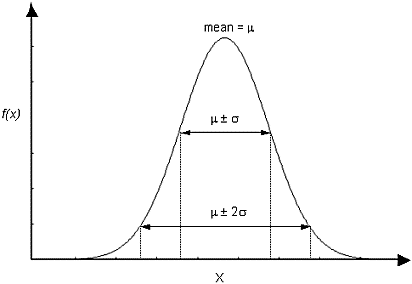
\includegraphics[width=\textwidth]{fig_dist_normal}
  \end{columns}
\end{frame}

\begin{frame}
  \frametitle{RSS — функция потерь}
  \centering
  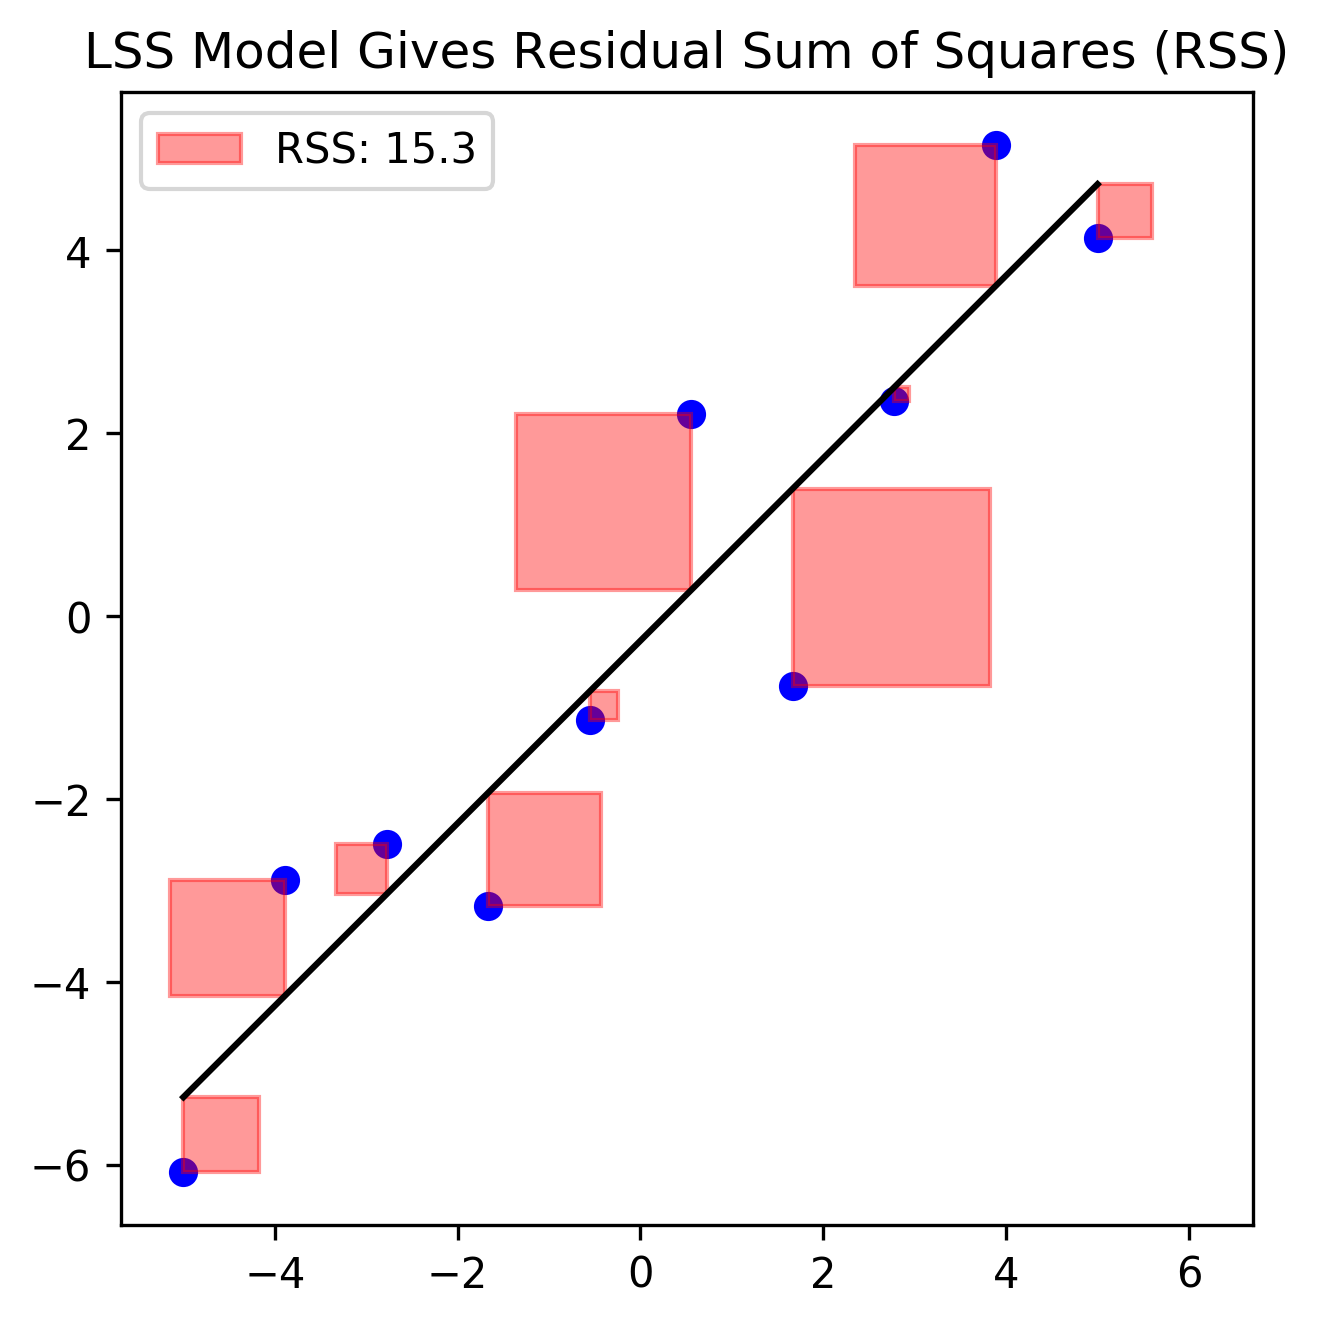
\includegraphics[height=.8\textheight]{mse}
\end{frame}

\begin{frame}
  \frametitle{Логистическая регрессия: бинарный классификатор}
  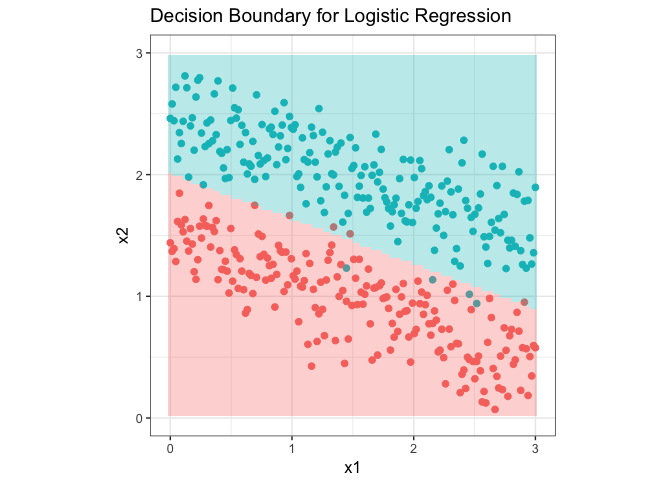
\includegraphics[width=\textwidth]{decision-boundary}
\end{frame}

\begin{frame}
  \frametitle{Логистическая регрессия: генеративная формулировка}
  \begin{columns}
    \column{.5\textwidth}
    \begin{equation}
      \begin{split}
        \label{eq:1}
        Y_i \sim \mathrm{Binomial}(1, p_i)\\
        \mathrm{logit}(p_i) = \alpha + \beta_1 x_1 + \beta_2 x_2 \\
        \mathrm{logit}(p_i) = \log\frac{p_i}{1-p_i}
      \end{split},
    \end{equation}
    где
    \begin{itemize}
    \item[$Y_i$] класс индивида i \{0,1\}
    \item[$p_i$] вероятность позитивного класса (1) для индивида i
    \end{itemize}
    \column{.5\textwidth}
    \includegraphics<1>[width=\textwidth]{Logistic-curve}
    \includegraphics<2>[width=\textwidth]{log-reg-acc}
  \end{columns}
  
\end{frame}

\begin{frame}
  \frametitle{Логистическая регрессия — функция потерь}
  \begin{equation}
    LS = - ( y log(p) + (1-y)log(1-p))
  \end{equation}
  \textbf{Примеры}:
  \begin{equation}
    \begin{split}
      \textbf<2>{y = 1 ; p = 0.8} \\
      LS = - ( 1 * \alert<2>{log(0.8)} + (1-1) * log(0.2)) = \\
      = \alert<2>{0.22}
    \end{split}
  \end{equation}
  \begin{equation}
    \begin{split}
      \textbf<3>{y = 0 ; p = 0.8} \\
      LS = - ( 0 * log(0.8) + (1-0) * \alert<3>{log(0.2)}) = \\
      = \alert<3>{1.6}
    \end{split}
  \end{equation}
\end{frame}


\section{Снижение размерности: Регуляризация}

\begin{frame}
  \frametitle{Underfitting/Overfitting}
  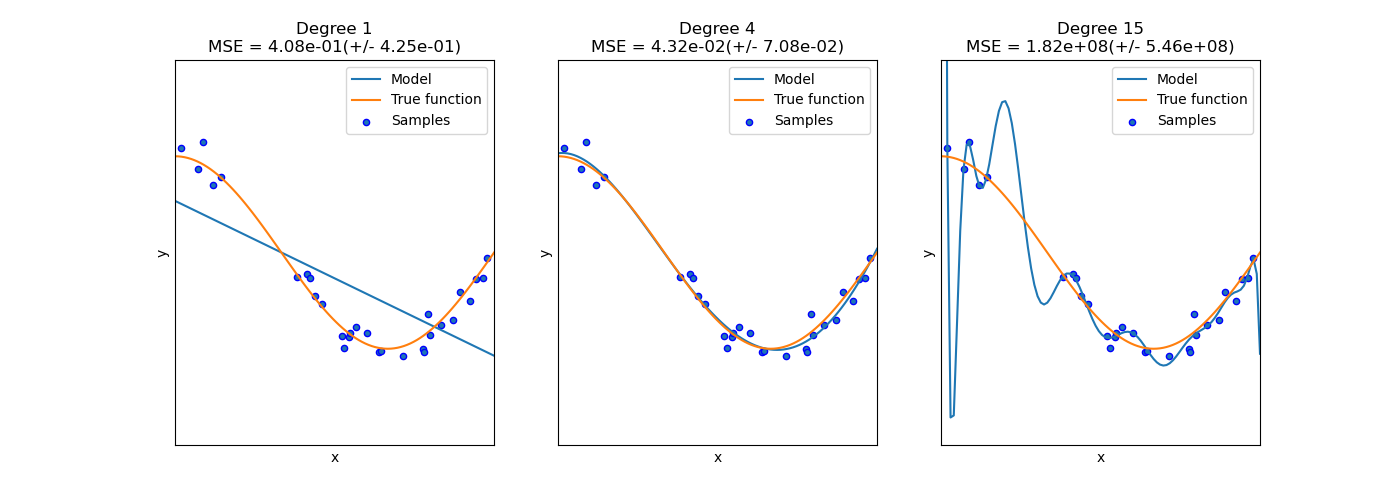
\includegraphics[width=\textwidth]{under_over}
\end{frame}

\begin{frame}
  \frametitle{Регуляризация}
  \includegraphics[width=\textwidth]{regularization-boundary}
\end{frame}

\begin{frame}
  \frametitle{Регуляризованная функция потерь}
  Обычная регрессия:
  \begin{equation}
    Loss = Error(y, \hat{y})
  \end{equation}
  L1 Loss (LASSO regression):
  \begin{equation}
    Loss = Error(y,\hat{y}) + \alert<2>{\lambda\sum|\beta_j|}
  \end{equation}

  L2 Loss (RIDGE regression):
  \begin{equation}
    Loss = Error(y,\hat{y}) + \alert<3>{\lambda\sum\beta_j^2}
  \end{equation}
\end{frame}

\begin{frame}
  \frametitle{Sceptical hamster}
  \centering
  
\includegraphics[height=.8\textheight]{sceptical-hamster}
\end{frame}


\end{document}
